\documentclass[12pt,fleqn]{article}\usepackage{../../common}
\begin{document}
Ders 1-18

Sonlu Öğeler, 2. Bölüm

Üzerinden geçelim, sistem zayıf form ile ise başlar. Önceki dersin sonunda
Galerkin fikrini tanıştırdık, sürekli diferansiyel denklem yerine onu ayrıksal
temsil etmeye uğraştık. Galerkin bunun için bazı deneme fonsiyonları kullanır
onlara $\phi_1,...,\phi_N$ diyelim, ayrıca test fonksiyonları da vardır (fakat
çoğunlukla test fonksiyonları ile deneme, yani $\phi$ ve $v$ fonksiyonları aynı
seçilir). Bugün işleyeceğimiz bu fonksiyonların nasıl seçildiği ve hazırlık
aşamasını gösterdikten sonra bunun verdiği $KU = F$ denklemin nasıl
çözüldüğü. $K$ nereden geliyor, $F$ nereden geliyor? $F$ bir şekilde alttaki
ikinci denklemin (oktan sonra) sağ tarafından geliyor, $K$ ise sol
tarafından.. Detayları şimdi göreceğiz.

$$
- \frac{\ud}{\ud x} \left( c(x) \frac{\ud u}{\ud x} \right) = f(x) \to
$$

$$
\int _{0}^{1} c \frac{\ud u}{\ud x} \frac{\ud v}{\ud x} \ud x =
\int _{0}^{1} f(x) v(x) \ud x
\mlabel{1}
$$

ki eger $u(1)=0$ ise $v(1) = 0$ (sinir sarti).

Sonlu ogeler metotunun (FEM) temeli $KU = F$. Ustteki denklemde okun sol tarafi
diferansiyel denklemimiz, sinir sartlari vs ile ``guclu formda'', oktan sonrasi
zayif form, ki onun da kendi sinir sartlari var. Sabit degiskenler guclu formdan
zayif forma geciyor, ama serbest degiskenler gecmiyor. $v$'yi $u$'dan olan ufak
sapmalar olarak gordugum icin eger $u$'yi sabitliyorsam $v$ de sabitleniyor.

Tum bunlari gorduk ama hala ayaklarimiz yere basmadi; bir cok fikirden
bahsettik, ama simdi daha gercek dunyaya baglanacagiz. Gercek dunya demek tabii
$\phi$'lerle alakali, hangi somut fonksiyonlari $\phi$ olarak sececegiz?

Acaba ornek bir $\phi$ ne olabilir? Mesela $x=2$ noktasinda tepe yapan bir
parcali lineer fonksiyon kullanabilirim,

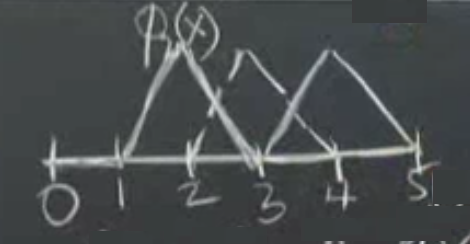
\includegraphics[width=10em]{compscieng_1_18_01.png}

Bu fonksiyona $\phi_2(x)$ diyelim, 1 ila 3 arasinda 2 uzerinde tepe yapiyor
diger yerlerde ya lineer egimi var, ya da degeri sifir. Her $\phi$ maksimum tepe
noktasi 1 olarak secilebilir. Onun sagindaki $\phi_3$ olabilir, benzer bir
fonksiyon sadece 3 degeri bazli tanimli. Buradaki ana amac sistemi basit ogeler
uzerinde insa etmek. FEM'in ana fikri budur; $\phi$ icin basit fonksiyonlar
kullan. Bu basitligin devami olarak $\phi$ ve $v$ fonksiyonlarini ayni sec.

Peki sinir noktalarinda ne olacak? Ustte serbest-sabit problemi cozecegim,
sol uc nokta serbest, sag uc nokta sabit (sinir tanimlanmis). 

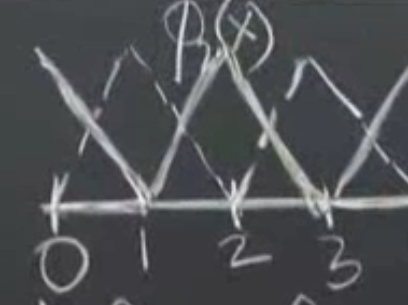
\includegraphics[width=10em]{compscieng_1_18_02.png}

Ustteki resme bakarsak, $x=0$ icin bir ``yarim sapka'' fonksiyonu tanimladim,
$\phi_0$ diyelim, ve eger diger ucgen fonksiyonlara tam sapka dersek bu da yarim
sapka. O noktada $\phi$ ve $v$'lerim kisitli degiller. Boylece elimde bes tane
deneme fonksiyonu oluyor, $\phi_0$, $\phi_1$, $\phi_2$, $\phi_3$, $\phi_4$.

Amac nedir? Yaklasik FEM cozumum $U(x)$'in ustteki basit sapka fonksiyonlarinin
bir kombinasyonu olmasini istiyorum.

$$
U(x) = U_0 \phi_0(x) + ... + U_4 \phi_4(x)
\mlabel{2}
$$

$U_0,..,U_4$ degerleri skalar, tek sayi.. onlar ilk basta bilinmeyen ``agirlik''
degerleri, $\phi$'leri belli sekilde carpacaklar ve bu carpimlarin toplami
yaklasik bir $u$ olacak.

Bu kombinasyonlar neye benzerdi acaba? 

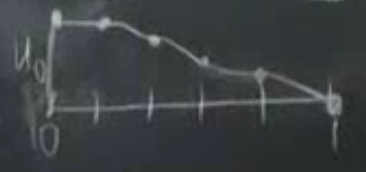
\includegraphics[width=10em]{compscieng_1_18_03.png}

Baslangictaki deger niye $u_0$? Cunku orada tum diger $\phi$ fonksiyonlari sifir
seviyesinde, hemen yandaki $\phi_1$ bile orada sifir ve maksimum $\phi$ deger 1
oldugu icin baslangic degeri $u_0$.

Bu arada Galerkin, ismini tasiyan yontemi bulurken, aklinda erismeye ugrastigi
belli bir cozum fonksiyonu vardi, ve sapka fonksiyonlarini oraya varmak icin
secmisti fakat modern FEM yaklasimlarinda, yazilimlarinda bir temel fonksiyonu
ilk bastan seceriz, problem hakkinda bir sey bilmesek bile. Sapka fonksiyonlari
bu fonksiyonlardan biridir.

Sonlu ogeler temel fonksiyonlari dugum noktalariyla baglantilidir, bu baglamda
sonlu farklilikler (finite differences) metotuna benzer (tabii FD ile esit
aralikla bolmek gerekir, FEM ile bu zorunluluk yok), ogeler dugum noktalarina
oturtuluyor. FEM ile sapka fonksiyonu ozelinde her dugum noktasindaki $u$
degerinin o noktadaki agirlik degeri ile ayni olmasini zorlamis oluyoruz; mesela
1 dugumundeki deger nedir? $u_1$! Cunku orada diger tum sapka fonksiyonlari
sifirdir, sadece $\phi_1$ degeri 1, toplanan tum terimler yokoluyor geriye
sadece $u_1 \phi_1 = u_1$ kaliyor.

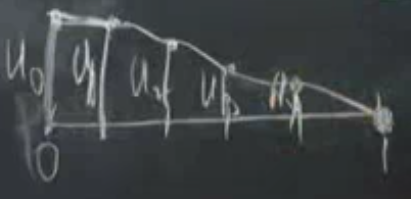
\includegraphics[width=10em]{compscieng_1_18_04.png}

FD benzerligi hakkinda, $KU=F$'i olusturdugumuzda onun bir FD denklemine oldukca
benzedigini gorecegiz, arada yapisal farklar var tabii, FD ile ayriksal
denklemleri biz tanimliyoruz, FEM ile sadece baz ogeleri seciyoruz denklemin
ne oldugunu Galerkin yontemi bize soyluyor.

Simdi bize lazim olan ustteki resimdeki her nokta icin ayri bir denklem, yani
toplam 5 tane denklem. Bu denklemler nereden gelecek? Kritik bir soru.

Bu denklemler zayif formdan gelecekler. Sunu yapiyorum, (1)'deki $u$ yerine
(2)'deki $U$'yu sokuyorum. Ayrica bir $v$ lazim, daha once $v(1)=0$ sarti takip
edilmek suretiyle herhangi bir $v$ olabilir demistik, ama simdi ayriksal forma
gectik, ben de $\phi_i$ fonksiyonlarini $V_i$ fonksiyonlarim icin kullanmaya
karar veriyorum. Boylece,

$$
\int _{0}^{1} c(x) \frac{\ud U}{\ud x} \frac{\ud V_i}{\ud x} \ud x =
\int _{0}^{1} f(x) V_i(x) \ud x
\mlabel{3}
$$

ki $i=0,1,2,3,4$. Boylece 5 tane denklem elde ediyorum, 5 tane $V$ ile ana
formulu ``test ediyorum''. Yani ustteki denklemi 5 tane $V$ icin farkli
sekillerle uretmis oluyorum. Iste 5 x 5 sistemim bu. Neler yaptim simdiye kadar?
Baz fonksiyonlarini sectik, onlari zayif forma sokuyoruz. $\ud U / \ud x$
agirlikli toplamdan geliyor (dikkat tum $V$'leri kullanarak), sonra
$\ud V_i / \ud x$ sokuyoruz, ve entegrali hesapliyoruz. FD durumunda bu
hesap yoktu, entegral hesabi yani, FEM ile var, esitligin hem saginda hem de
solunda.  Esitligin sagindaki entegral her $V_i$ icin bize bir $F_i$ verecek,
yani $F$ vektorunun bir satirini. Tabii $K$ matrisi esitligin solundan
bir sekilde cikacak, nasil birazdan gorecegiz.

Ornek 1

Sag tarafa bakalim once, mesela $i=0$ icin, $f(x)=1$ olsun (ornege gore
boyle) bu durumda $\int_{0}^{1} 1 \cdot V_0(x) \ud x$ entegrali ne
olur? Entegral bir alan hesabidir hatirlarsak, o zaman 

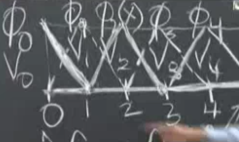
\includegraphics[width=10em]{compscieng_1_18_05.png}

$V_0$ ustteki ilk yarim sapka, o ucgenin alani, eger $x$ ekseni esit araliklarla
bolmussek ve her aralik $\Delta x$ ise, $(\Delta x \cdot 1) / 2 = \frac{\Delta x}{2}$.

Dikkat 0 ila 1 arasi entegral ustteki resimdeki tum yatay ekseni kapsar,
0,1,2,..  indisleri kafa karistirmasin. O indisler $x=0$ ile $x=1$ arasini
indisliyor. O zaman 0 ile 1 arasi entegral tum $V$'lerin oldugu alan uzerinden
alinir, fakat biz her seferinde birini sectigimiz icin onun alanini hesaplamis
oluyoruz cunku mesela $V_0$ tanimlandigi yer sonrasinda sifir degerinde.

$i=1$ icin ne olur? $\int_{0}^{1} 1 \cdot V_1(x) \ud x$, ucgen tabani
$2 \Delta x$,  carpi 1, sonuc $\Delta x$. diger $V$ degerleri benzer sekilde,
o zaman $F$ vektor su sekilde,

$$
F = \left[\begin{array}{c}
1/2 \\ 1 \\ 1 \\ 1 \\ 1
\end{array}\right]
$$

$K$ icin hazir miyiz? Anahtar bolum orasi.

(3) formulunun tum sol tarafi $KU$'yu vermeli.. Satir satir gidelim, mesela
sifirinci denklem hangisi? $i=0$ oldugu zaman, yani $V_0$ kullanilan, zayif
formu $V_0$ ile test ettigimiz durumdur. Her seyi acarak yazarsak,

$$
\int _{0}^{1} c(x)
\left( U_0 \phi_0' + ... + U_4 \phi_4'  \right)
\frac{\ud V_0}{\ud x} \ud x = F_0 = \Delta x \cdot \frac{1}{2}
$$

Su ana kadar eldekileri matris formunda yazarsak,

$$
\left[\begin{array}{rrrrr}
 & & & & \\
 & & & & \\
 & & & & \\
 & & & & 
\end{array}\right]
\left[\begin{array}{r}
U_0 \\ U_1 \\ U_2 \\ U_3 \\ U_4
\end{array}\right] =
\left[\begin{array}{r}
F_0 \\ F_1 \\ F_2 \\ F_3 \\ F_4
\end{array}\right]
$$

Bos matrisin ilk satirini $V_0$'yi kullanarak yapacagim entegral hesabindan elde
edecegim. Daha kolay baslayalim, ilk satirin sol ilk hucresine ne gelir?
$K_{00}$ diyelim, oradaki deger $U_0$'i carpiyor degil mi ve bir sekilde
entegralinin alinmasi lazim.. Soyle olabilir mi?

$$
K_{00} = \int _{0}^{1} c(x) \phi_0' V_0' \ud x
$$

$c(x)$ icin simdilik 1 kabul edelim. Fakat eger 1 olmasaydi daha cetrefil bir
fonksiyon olsaydi? Icinde $c(x)$ olan bircok entegrali ustteki gibi hesaplamak
lazim, ve bu hesaplarin kesin olmasi gerekmeyebilir, yani bu entegralleri
yaklasik olarak hesaplasak ta yeterli olabilir. Sonucta diger her seyi yaklasik
yapiyoruz degil mi? Belli noktalar uzerinden yaklasik bir temsil yaratiyoruz
vs.. Bu cercevede eger ustteki turden entegralleri hesabin tumunu bozmayacak
seviyeye yetecek kesinlik3te hesaplayabilirsek, isimizi halletmis oluruz. $c(x)$
1 olunca tabii ki kesin cozumu bulacagiz ama diger tur durumlar icin aklimizda
olsun.

Hesabin kendisine gelelim. $\phi_0'$ nedir? Bu arada $\phi$'leri $V$ ile ayni
sectigimiz icin $\phi_0' = V_0'$ ve her iki turev ustteki resimdeki bastaki
yarim ucgenin egimi. Egitim dikey artis bolu yatay artis, yatay kisim $\Delta
x$, o zaman 1'inci dugume kadar $- 1 / \Delta x$, sonrasi sifir.

Bu vurgulanmasi gereken bir noktaya goturuyor, fonksiyonlarimiz yerel / lokal.
Bu ne demek? Eger $\phi_1'$ turevini $V_4'$ tureviyle entegre etseydim ($K$
matrisinde 4'uncu satir ile 1'inci kolon degeri yani) ne olacakti? Sifir
olacakti. Niye? Cunku bu fonksiyonlar yerel, 0'inci ve 4'uncu dugumlerden uzakta
degerleri sifir, sifir olmadiklari yerler cakismiyor. Simdi bu dinamigi tum
matris icin dusunursek ne kadar az cakisma yeri oldugunu gorebiliriz. Herhangi
bir $\phi$ mesela, tabii ki kendisiyle cakisir ve yanindaki komsularla biraz
cakisir. Ama daha ilerisiyle ortusmesi yoktur. Bu bize $K$ icin üçlü köşegen bir
matris verecek, uc ogeli kosegen bantinda degerler olacak, geri kalan her yer
sifir.

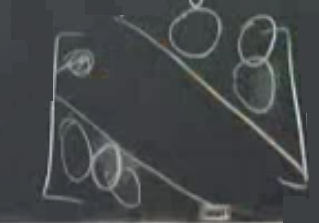
\includegraphics[width=10em]{compscieng_1_18_06.png}

$K_{00}$ hesabina donelim, $c(x)=1$, $\phi_0' = -1/\Delta x$, $V_0'$ ayni deger,
ve entegre ettigimizi unutmayalim, 0 ile 1 arasi ama aslinda 0 ile $\Delta x$
arasi cunku sadece oraya kadar degerler var, o zaman $K_{00} = 1/\Delta x$
oluyor.

Peki

$$
K_{11} = \int _{0}^{1} c(x) \phi_1' V_1' \ud x
$$

$\phi_1$ egimi nedir? Bu sapka fonksiyonu tam, $\Delta x$'e kadar yukari
cikiyor sonra asagi iniyor, o zaman

$$
\phi_1' = V_1' =
\left\{ \begin{array}{rc}
1/\Delta x & 0 < x \le \Delta x \\
-1/\Delta x & \Delta x < x \le 2\Delta x 
\end{array} \right.
$$

$\phi_1'$ ve $V_1'$ carpimi her iki bolum icin $1/\Delta x^2$ verir. Peki
$K_{11}$ entegral sonucu ne o zaman? $2 \Delta x$ degil mi? Cunku bu sefer
entegral sinirlarina dikkkat, 0 ile $2\Delta x$ arasinda. 

$$
K_{11} = \int _{0}^{2\Delta x} c(x) \phi_1' V_1' \ud x = 2\Delta x
$$












[devam edecek]



\end{document}

